\documentclass[aspectratio=169]{beamer}
\usetheme{Madrid}
\usecolortheme{default}
\usepackage{booktabs}
\usepackage{graphicx}
\usepackage{array}

\title[Model Merging SAE Checkpoint]{Model Merging SAE Checkpoint}
\subtitle{Qwen generated-trace SAE result and Gemma candidate promotion}
\author{Gavin model-merging project}
\date{2026-05-22}

\begin{document}

\begin{frame}
  \titlepage
\end{frame}

\begin{frame}{Current Question}
  \begin{block}{Research gate}
  Can a sparse or transcoder basis explain merge-induced safety loss better than
  raw activations, PCA, top-coordinate patches, and module patching?
  \end{block}

  \vspace{0.5em}
  The value-action project taught us to stop trusting a sparse basis until it
  passes matched baselines and causal completeness checks.

  \vspace{0.5em}
  Today's checkpoint:
  \begin{itemize}
    \item Qwen: generated-token SAE training changes the family repaired, but still fails the full v0 gate.
    \item Gemma: a cleaner abliterated pair with public GemmaScope bases now passes behavior and RQ0 activation screens.
  \end{itemize}
\end{frame}

\begin{frame}{Qwen Result: Distribution Matters, But Gate Still Fails}
  \centering
  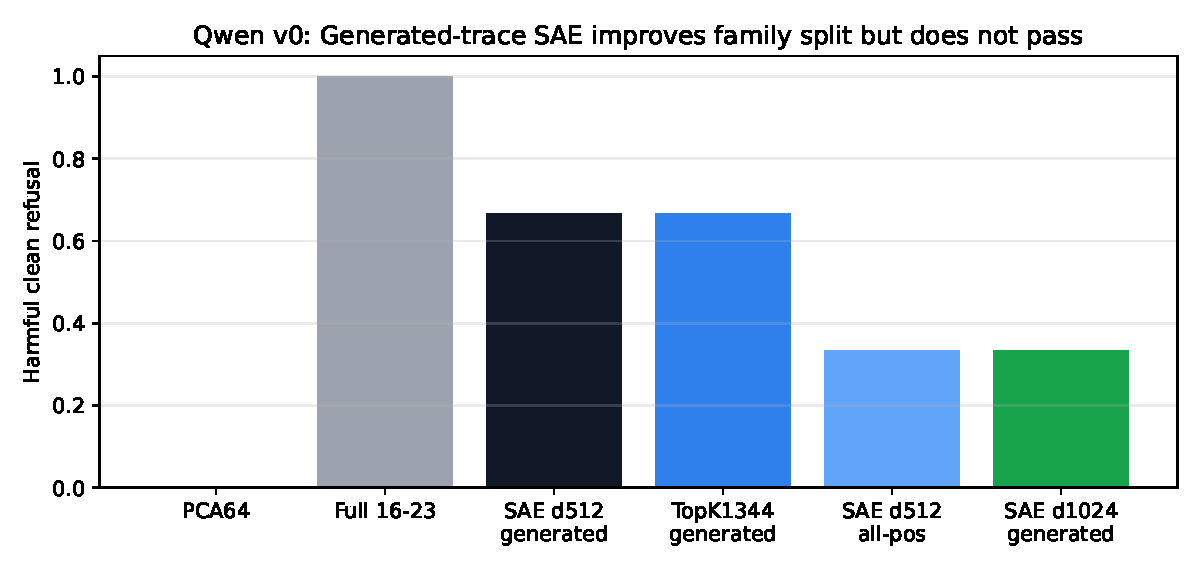
\includegraphics[width=0.86\linewidth]{figures/qwen_generated_trace_harmful_clean.pdf}

  \vspace{0.4em}
  \small
  Generated-token d512 repairs one-time-code and permission-slip, unlike the earlier
  teacher-forced SAE. Tracking still fails, and full donor 16-23 remains the only
  v0-complete repair.
\end{frame}

\begin{frame}{Qwen Interpretation}
  \small
  \begin{tabular}{p{0.34\linewidth} p{0.56\linewidth}}
  \toprule
  Finding & Meaning \\
  \midrule
  High SAE EV still fails behavior & Reconstruction quality is not causal completeness. \\
  Generated-token d512 reaches 0.667 & Token distribution mismatch was partly real. \\
  All-position d512 falls to 0.333 & Adding prompt rows does not automatically capture tracking. \\
  Tracking remains unrepaired & Next sparse attempt should be family/pathway specific. \\
  \bottomrule
  \end{tabular}

  \vspace{1em}
  Decision: do not keep widening vanilla Qwen residual SAEs as the main path.
  The next Qwen sparse work should be family-specific, position-specific, or
  transcoder-style.
\end{frame}

\begin{frame}{Gemma Candidate: Cleaner Model Pair}
  \small
  \begin{tabular}{lcccc}
  \toprule
  Model & Refusal pass & Harmful clean & Benign helpful & Clean gen \\
  \midrule
  \texttt{google/gemma-2-2b-it} & yes & 1.000 & 1.000 & 1.000 \\
  \texttt{IlyaGusev/gemma-2-2b-it-abliterated} & no & 0.000 & 1.000 & 1.000 \\
  \bottomrule
  \end{tabular}

  \vspace{1em}
  Both models have matching Gemma2 configs: 26 layers, hidden size 2304,
  intermediate size 9216, 8 attention heads, 4 KV heads, vocab size 256000.

  \vspace{0.5em}
  This gives us a larger and cleaner safety-behavior diameter than the current
  tiny Qwen v0 benchmark, with a stronger public sparse-basis ecosystem.
\end{frame}

\begin{frame}{Gemma RQ0: Harmful-Specific Activation Drift}
  \centering
  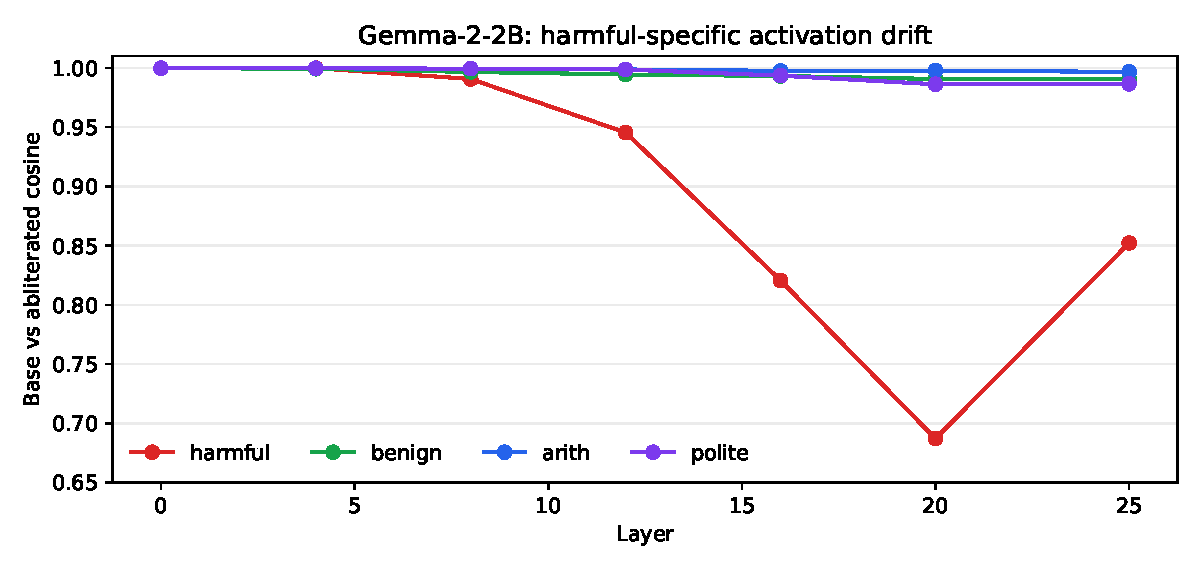
\includegraphics[width=0.86\linewidth]{figures/gemma_activation_similarity.pdf}

  \vspace{0.4em}
  \small
  At layer 20, base vs abliterated cosine is 0.687 on harmful prompts but 0.991
  on benign prompts. Arithmetic and polite prompts stay near aligned.
\end{frame}

\begin{frame}{Decision}
  \begin{block}{Keep Qwen, promote Gemma}
  Qwen remains useful for the distributed-residual story. Gemma becomes the next
  candidate branch for public SAE/transcoder analysis, but only after causal
  patching establishes a repair target.
  \end{block}

  \vspace{0.5em}
  Next steps:
  \begin{enumerate}
    \item Run Gemma module and activation patching to localize refusal repair.
    \item Compare Gemma low-rank and top-coordinate baselines.
    \item Only then load GemmaScope SAEs/transcoders for basis validation.
    \item Keep Qwen sparse work limited to family-specific or transcoder-style tests.
  \end{enumerate}
\end{frame}

\begin{frame}{Provenance}
  \small
  \begin{itemize}
    \item Qwen generated-trace interpretation: \texttt{stage3/results/qwen1\_5b\_residual\_sae\_generated\_full\_v0/}
    \item Gemma behavior screen: \texttt{stage0/results/candidate\_screens\_gemma2\_2b\_abliterated\_20260522\_clean/}
    \item Gemma RQ0 screen: \texttt{stage1/results/gemma2\_2b\_abliterated\_rq0/}
    \item Value-action lesson memo: \texttt{docs/VALUE\_ACTION\_LESSONS\_FOR\_MODEL\_MERGING.md}
    \item Commits pushed: \texttt{5114edd}, \texttt{9ebfbd0}
  \end{itemize}
\end{frame}

\end{document}
